\section{Background}

\subsection{LLM Inference Service Architecture}

A typical LLM service separates application orchestration from model execution, as shown in Fig.~\ref{fig:inference_engine}. Upper-layer applications construct prompts, retrieve context, or invoke external tools and data sources; the orchestration layer packages this information into a generation request and consumes the returned tokens. The \emph{inference engine} is the serving and runtime stack that processes the request on one or more compute devices. It does not include model training or application-side logic such as retrieval-augmented generation.

\begin{figure}[t]
    \centering
    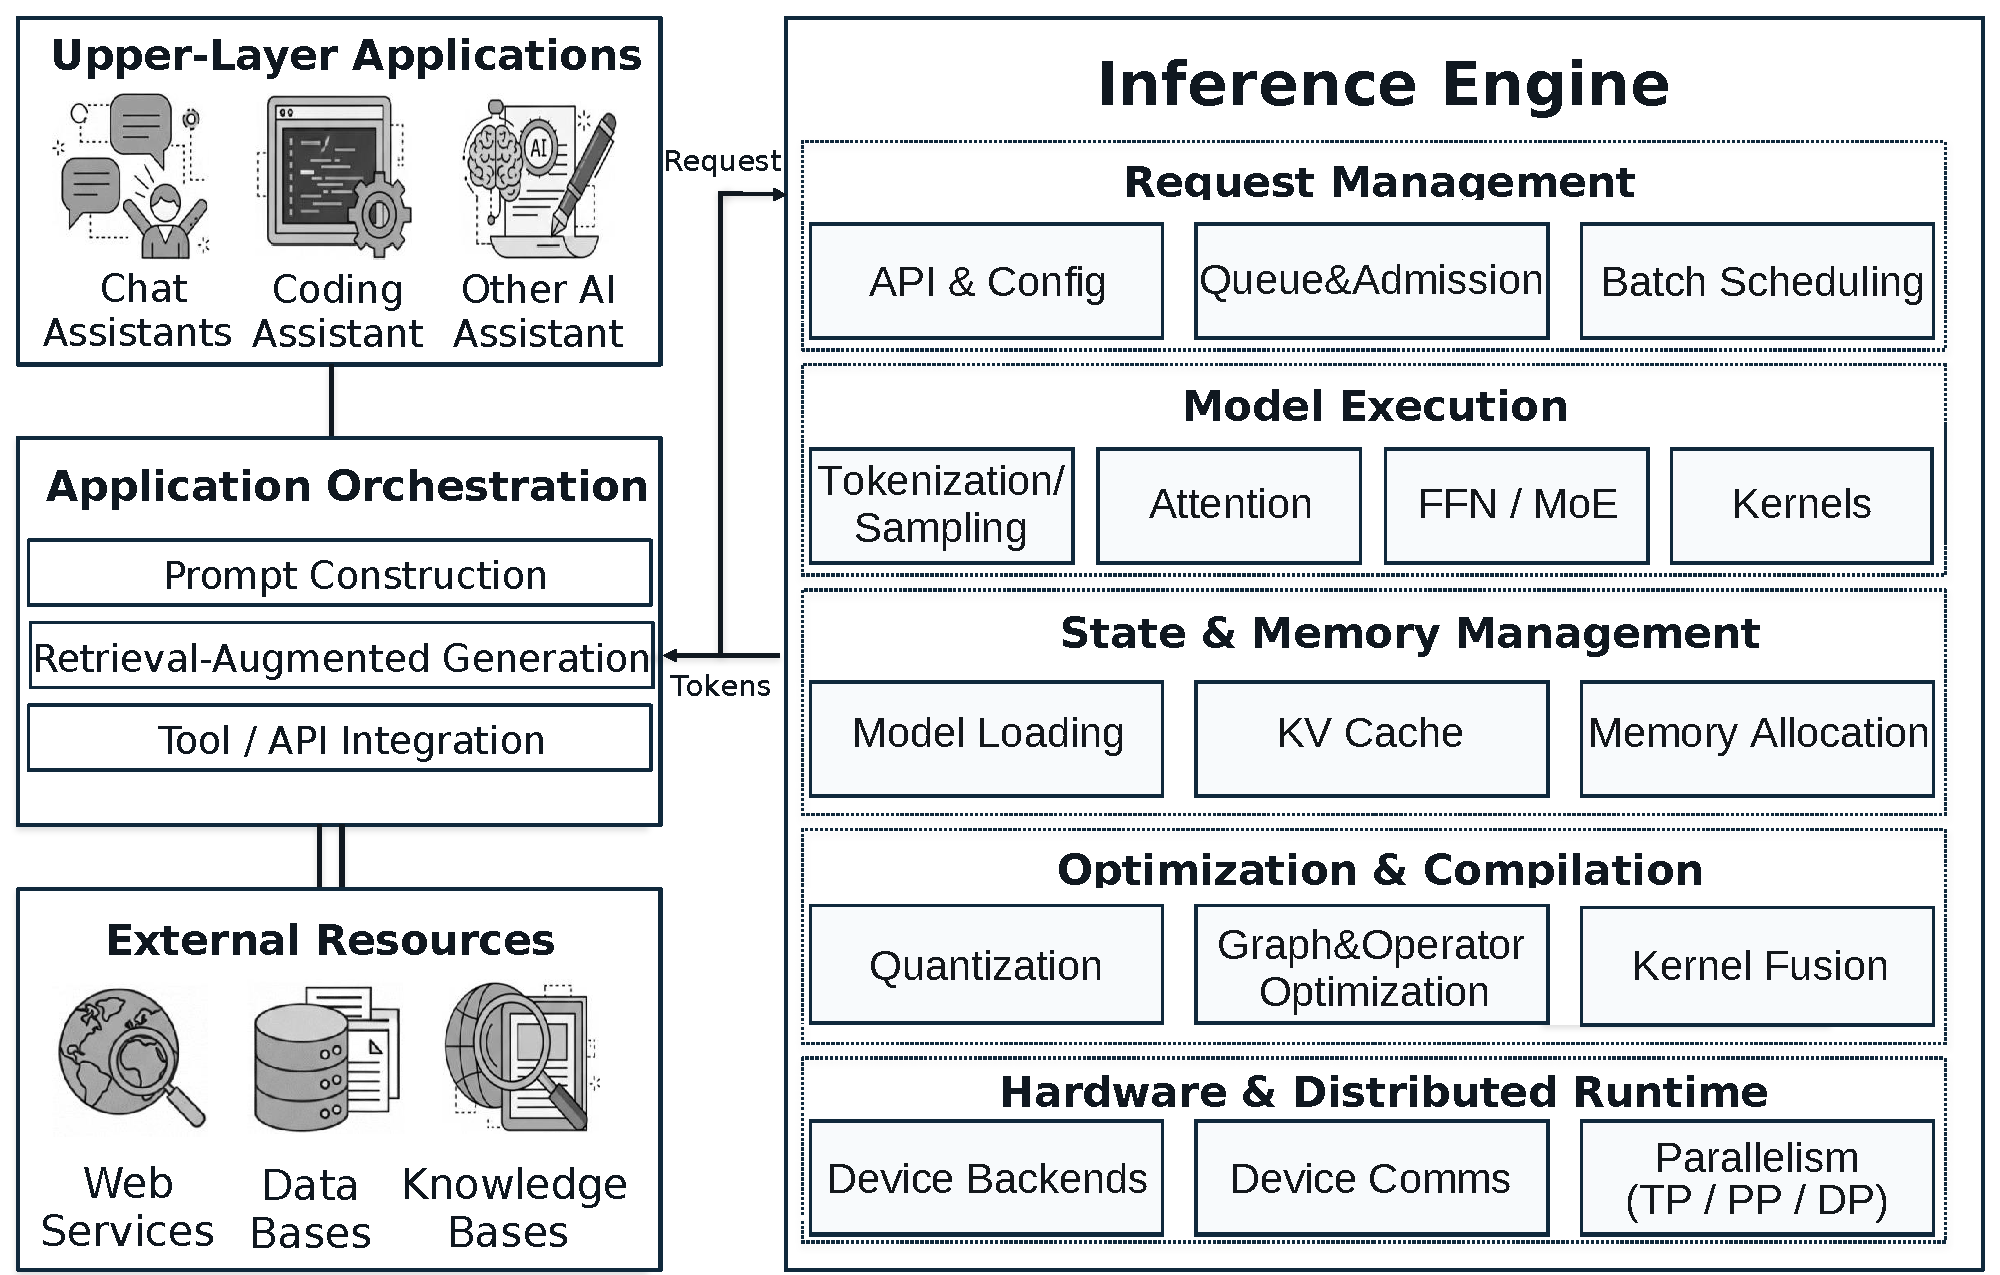
\includegraphics[width=0.95\linewidth]{fig/inference_engine.pdf}
    \caption{Overview of a typical LLM inference service. Application orchestration prepares generation requests and interacts with external resources, while the inference engine manages requests, model execution, state and memory, optimization, and heterogeneous hardware.}
    \label{fig:inference_engine}
\end{figure}

The online path begins with \emph{request management}. This region parses API inputs and generation configurations, validates whether a request can be served, and places admitted requests into a queue. The scheduler then selects requests for each iteration and forms batches from sequences that may arrive at different times and have different lengths. Iteration-level and continuous scheduling improve device utilization by allowing completed requests to leave and new requests to join without waiting for an entire batch to finish~\cite{yu2022orca,kwon2023pagedattention}. Beyond batching within one model, AlpaServe uses model parallelism and placement to multiplex bursty multi-model workloads, while SpotServe dynamically reconfigures distributed inference under instance preemption~\cite{li2023alpaserve,miao2024spotserve}.

Selected requests enter \emph{model execution}. Tokenization converts input text into model tokens, while sampling converts output scores into the next generated token. Between these steps, the engine invokes embeddings, attention, feed-forward or mixture-of-experts layers, and output operators through optimized kernels and software backends. Transformer attention has quadratic time and memory complexity in the sequence length~\cite{vaswani2017attention}; optimized kernels such as FlashAttention-2 reduce memory traffic and improve parallel work partitioning~\cite{dao2024flashattention2}. Execution depends on \emph{state and memory management}, which loads model weights, maintains the key--value (KV) cache, and allocates memory as sequences grow. CacheGen further treats cached state as a compressed stream whose transfer policy adapts to network bandwidth~\cite{liu2024cachegen}. \emph{Optimization and compilation} apply techniques such as low-bit quantization~\cite{lin2024awq}, graph rewriting, operator optimization, and kernel fusion; QServe illustrates how weight, activation, and KV-cache precision must be co-designed with GPU kernels to obtain serving speedups~\cite{lin2025qserve}. The \emph{hardware and distributed runtime} maps the resulting computation to CPUs, GPUs, or NPUs and coordinates communication and parallel execution~\cite{aminabadi2022deepspeed}. Modern engines organize these responsibilities differently~\cite{kwon2023pagedattention,zheng2024sglang,zhong2024distserve,pope2023scaling,park2026inferenceengines}; Fig.~\ref{fig:inference_engine} therefore presents functional regions rather than fixed module boundaries.

Within this architecture, autoregressive generation proceeds in two execution phases with different workloads. During \emph{prefill}, the engine processes the prompt and materializes the initial KV-cache state. During \emph{decoding}, it repeatedly schedules an iteration, executes the model for the current token position, updates the cache, and samples the next token until a stopping condition is met~\cite{vaswani2017attention}. Prefill is primarily compute-bound, whereas decoding is commonly memory-bandwidth-bound~\cite{patel2024splitwise,lin2024awq}. A serving engine interleaves these operations across concurrent requests, whose arrival times, prompt lengths, and output lengths are generally different. It must consequently coordinate scheduling with KV-cache allocation, device capacity, and---for distributed deployments---worker communication~\cite{yu2022orca,kwon2023pagedattention,agrawal2024sarathi,zhong2024distserve}. Request control, model execution, memory state, optimization, and hardware support therefore interact throughout the lifetime of a request rather than forming an isolated sequence of steps.

Fault location does not always match repair extent. A wrong scheduling decision may become visible only during model execution, while a backend-specific operator fault may also require changes to dispatch logic, tests, and configuration. We therefore record the faulty architectural layer separately from the code entities modified by the fix. Layer labels give a common functional view of projects with different source-tree structures. File-, function-, and patch-level measures show where repairs recur and how far they reach. This distinction avoids treating every modified file as a fault location without losing the coordination visible in the complete patch.
